\chapter{Спектральная диагностика~низкотемпературной плазмы газового разряда}
%\chapter{СПЕКТРАЛЬНАЯ ДИАГНОСТИКА НИЗКОТЕМПЕРАТУРНОЙ ПЛАЗМЫ ГАЗОВОГО РАЗРЯДА}
\label{cha:ch_1}
\section{Кинетика заселения возбужденных атомных состояний в плазме}
Спектры излучения газоразрядной плазмы определяются населенностью \math{N_j}$ соответствующих возбужденных атомных уровней \math{E_j}$.
Тогда интенсивность соответствующей атомной спектральной линии составит:
\begin{equation}
    I_{ji} = A_{ji}h\nu_{ji}⋅N_j
\end{equation}
где \math{A_{ji}}$  - коэффициент Эйнштейна для перехода \math{j → i}$, \math{N_j}$ - населенность возбужденного уровня \math{j}$.

Таким образом, задача спектральной диагностики плазмы сводится к построению теоретических моделей, связывающих
параметры плазмы (в первую очередь, концентрации электронов \math{n_e}$ и их температуру \math{T_e}$) с интенсивностями спектральных
линий \math{I_{ji}}$. Выбор той или иной модели зависит от параметров плазмы: ее химического состава, плотности,
степени ионизации и равновесности. В данной работе экспериментально и теоретически исследуется стационарная сильно
неравновесная плазма положительного столба слаботочного газового разряда постоянного тока (\math{I_{DC}~=~1~мА}$)
в неоне при давлении \math{P~=~50~Па}$, причем степень ионизации плазмы α очень мала (\math{\alpha~\sim~10^{-8}}$).
Выбор этих параметров обуславливается практическим случаем, рассматриваемым в этой работе.
\begin{figure}[t]
    \begin{center}
         \subfloat[\label{sub:fig11a}]{
           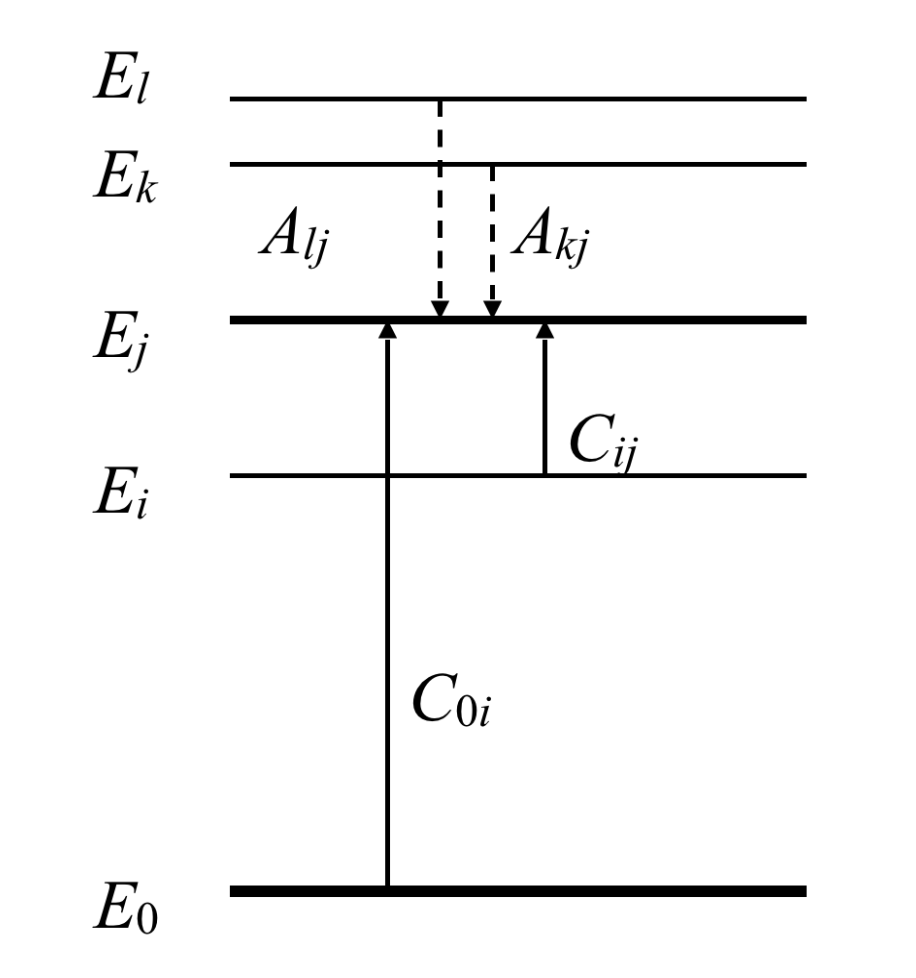
\includegraphics[width=0.35\textwidth]{figures/fig11a}
         }
         \hspace{0.05\columnwidth}
         \subfloat[\label{sub:fig11b}]{
           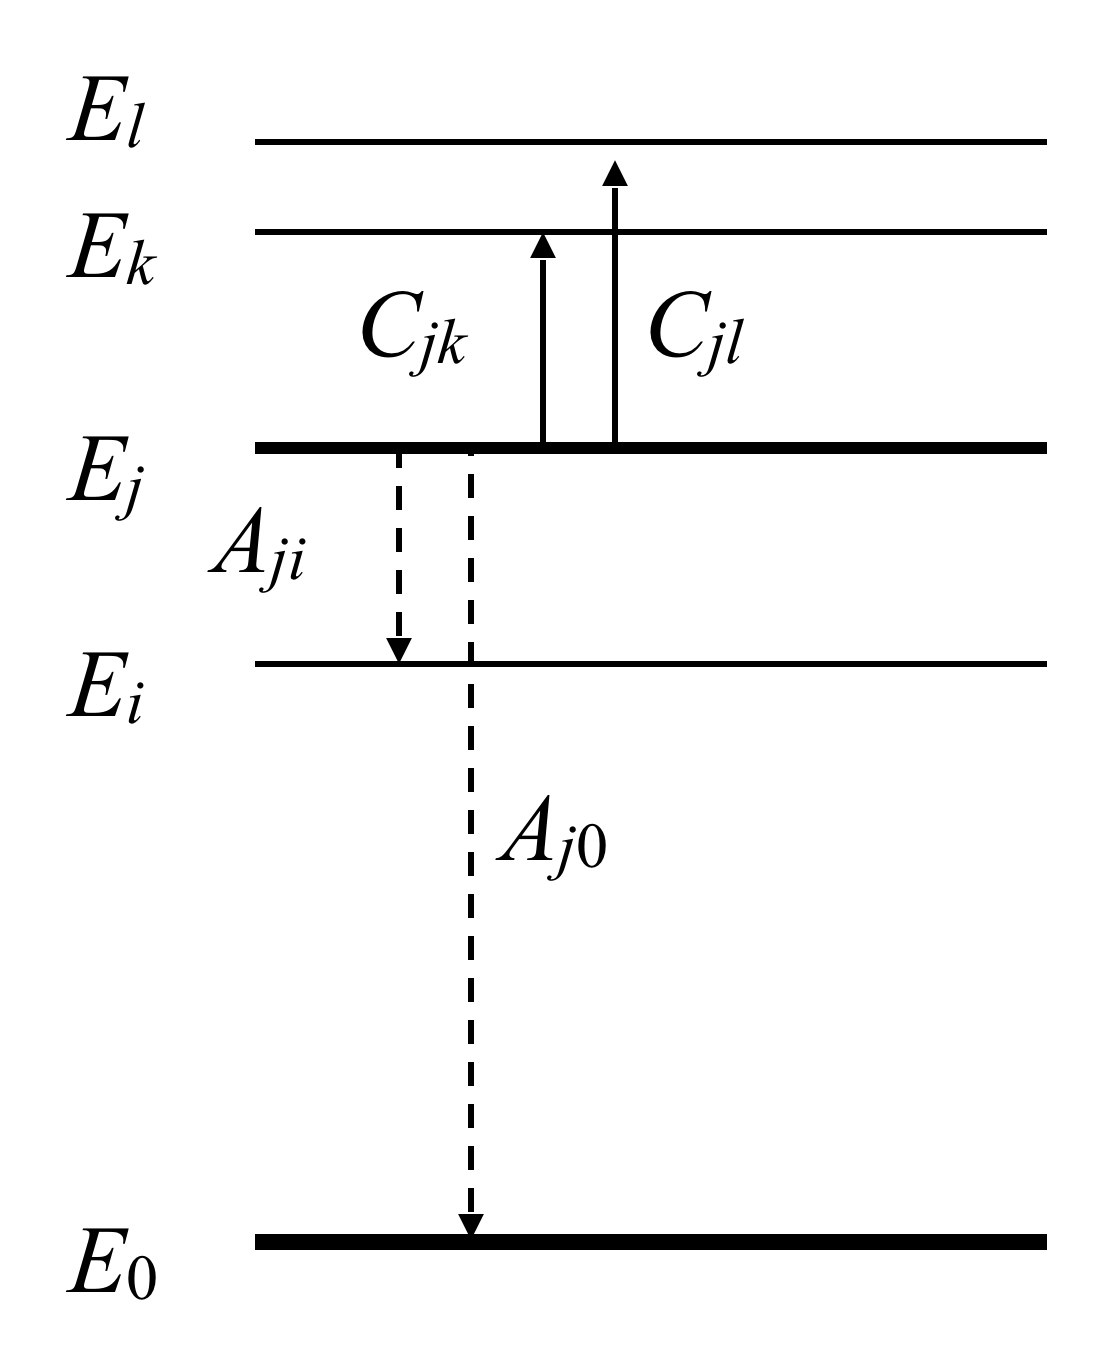
\includegraphics[width=0.305\textwidth]{figures/fig11b}
         }
         \caption{Схема основных процессов уровня: \pt(a) заселение, \pt(b) расселение.}
         \label{fig:fig11}
    \end{center}
\end{figure}

Населенность \math{N_j}$ уровня \math{E_j}$ в стационарном случае определяется балансом процессов его заселения
и расселения. Схема основных процессов заселения уровня \math{E_j}$ представлена на рис.~\ref{fig:fig11}~\subref{sub:fig11a}.
Основным процессом заселения рассматриваемого уровня \math{E_j}$ является его заселение прямым
электронным переходом с основного состояния \math{E_0}$ и с метастабильного \math{E_i}$.

Скорости процессов \math{C_{0j}}$ и \math{C_{ij}}$ определяются соотношениями:
\begin{equation}C_{0j} = \sqrt{2 \over m_e} \int_{E_j}^{\infty} \sigma_{0j}(E) f_e(E) \sqrt{E} dE\end{equation}
и
\begin{equation}C_{ij} = \sqrt{2 \over m_e} \int_{E_j - E_i}^{\infty} \sigma_{ij}(E) f_e(E) \sqrt{E} dE\end{equation}
соответственно, где …

Сечения \math{\sigma_{0j}(E)}$ и \math{\sigma_{ij}(E)}$ расчетные и экспериментальные, можно найти в литературе
или базе данных NIST [ССЫЛКА НА ИСТОЧНИК]. Типичный вид сечений представлен на рис. \ref{fig:fig12}.
Что касается вида ФРЭ, то она сильно зависит от параметров плазмы. При высоких давлениях ФРЭ приближается
к максвелловской функции. Однако, при низких давлениях плазма сильно неравновесна, и вид функции ФРЭ должен
быть определен дополнительными методами. Кроме столкновительного заселения уровень \math{E_j}$ заселяется
также путем радиационного распада верхних \math{k}$-уровней \math{E_k~>~E_j}$ cо скоростью \math{A_{kj}}$ при \math{k > j}$.
Значения \math{A_{kj}}$ также табулированы в базе данных NIST.
\begin{figure}[t]
  \centering
  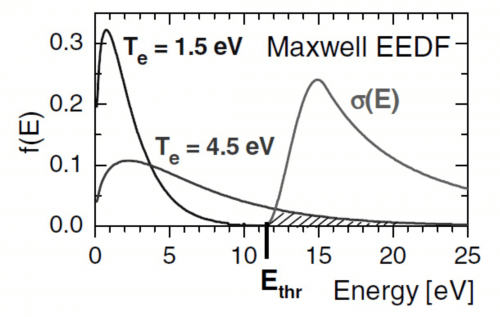
\includegraphics[width=8cm]{figures/fig12}
  \caption{Типичный вид сечения \math{\sigma}$ и максвелловской ФРЭ. \math{T_e}$ - температура электронов, \math{E_{thr}}$ - пороговая энергия..}
  \label{fig:fig12}
\end{figure}

Схема основных процессов расселения уровня \math{E_j}$ представлена на рис.~\ref{fig:fig11}~\subref{sub:fig11b}.
Этими процессами также являются явления спонтанного распада возбужденных уровней и столкновительные процессы,
индуцированные свободными электронами.

Приравняв скорости заселения и расселения уровня \math{E_j}$, мы получим уравнение относительно ФРЭ \math{f_e(E)}$.
Это уравнение является некорректной задачей и для ее решения необходимы дополнительные данные о виде ФРЭ.
Эти данные могут быть получены путем решения кинетического уравнения Больцмана для соответствующих условий.

\section{Уравнение Больцмана для ФРЭ в положительном столбе газового разряда постоянного тока.}

Газовые разряды представляют собой крайне неравновесную систему, в которой средняя энергия электронов (температура)
на два порядка превышает температуру газа. Функция распределения электронов (ФРЭ) характеризуется нагревом
электронов электромагнитными полями и столкновениями их с нейтральными атомами, почти во всех случаях это распределение
отклоняется от равновесного (Максвелловского). Решение кинетического уравнения Больцмана для ФРЭ является
важнейшей задачей для точного моделирования плазмы, так как многие явления невозможно правильно понять
без кинетического анализа. Уравнение Больцмана существенно можно упростить из-за большого различия масс электронов и атомов.
В силу данного различия, затухание энергии электронов в упругих столкновениях с атомами происходит гораздо медленнее,
чем затухание импульса электронов (\math{m_e \ll M_a}$). Как следствие, ФРЭ в скоростном пространстве может быть представлена как сумма
большой изотропной \math{f_0}$ и малой анизотропной частей \math{f_1}$.

Выделяют три существенно различных случая. Первый случай, когда величины \math{P L \gg 1}$ и \math{{E P} \ll 1}$, где
\math{P}$ - давление газа, \math{L}$ - характерный размер плазмы, \math{E}$ - электрическое поле, а
пространственные градиенты \math{f_0}$ и \math{f_1}$ малы и определены локальными значениями электрического поля,
электронной плотности и составом плазмы. Тогда электроны могут быть описаны уравнениями жидкости с коэффициентами переноса,
полученными из локальной (не Максвелловской) ФРЭ. Обычно через уравнение Больцмана решают задачу нахождения
коэффициентов переноса и скоростей протекания реакции для данного приближения.

Второй случай соответствует столкновительной плазме, где характерный размер плазмы \math{L}$ значительно больше средней длины
свободного пробега электронов \math{\lambda}$, но сравним с длиной релаксации энергии электрона \math{\lambda_\epsilon}$.
В этом нелокальном режиме изотропная часть ФРЭ \math{f_0}$ в заданной точке зависит не только от электрических полей в этой точке,
но и от свойств плазмы в окрестности точки размера (эффект памяти), а анизотропная часть \math{f_1}$ является лишь функцией
электрического поля \math{E}$. В этом столкновительном режиме плазма не может быть описана гидродинамикой.

В третьем случае, при дальнейшем уменьшении \math{P L}$, средняя длина свободного пробега электрона будет сравнима c характерным размером плазмы
(\math{\lambda \sim L)$. В этом почти бесстолкновительном случае анизотропная часть в точке определяется не только
значением напряженности электрического поля в этой точке, но и профилем электрического поля вдоль траектории электрона.
В результате локальная зависимость между плотностью тока и электрическим полем (закон Ома) становится недействительной \cite{Kolobov}.

Плазма тлеющего разряда низкого давления имеет сильно неравновесный характер. Рождение заряженных частиц происходит
преимущественно в объемных процессах, а гибель на стенках разрядной камеры. Энергию электроны приобретают,
разгоняясь в электрическом поле, а теряют в упругих и неупругих столкновениях. Количественное описание этих процессов
возможно только на кинетическом уровне \cite{Zobnin}.

В данной работе положительный столб газового разряда находится под низким давлением порядка 40~Па и имеет диаметр трубки 30~мм (см. раздел \ref{sec:sec_31}),
а значит для описания кинетических процессов с помощью уравнения Больцмана необходимо пользоваться почти бесстолкновительным приближением.

Кинетическое уравнение Больцмана представляет собой интегродифференциальное уравнение, описывающее эволюцию функции
распределения частиц в шестимерном (6-D) фазовом пространстве. Данное уравнение было выведено Людвигом Больцманом в 1872 г.
Оно до сих пор остается основой кинетической теории газов и оказывается плодотворным не только для исследования
классических газов, которые имел в виду Больцман, но - при соответствующем обращении - и для излучения переноса
электронов в твердых телах и плазме \cite{Cherchin'yani}. В общем виде оно выглядит следующим образом:

\begin{equation}
    {\partial f_e \over \partial t} + (\vec{v}, \vec{\Delta}_r) f_e + (\vec{a}, \vec{\Delta}_v) f_e = I
\end{equation}
где \math{f_e = f_e(\vec{r}, \vec{v}, t)}$~--~функция распределения электронов,
\math{\vec{r}}$~--~вектор положения в физическом пространстве, \math{\vec{v}}$~--~вектор скорости,
\math{\vec{a}}$~--~вектор ускорения, \math{t}$~--~время, \math{I}$~--~интеграл столкновений,
является интегральным оператором в пространстве скоростей, описывающим столкновения между частицами.

%{e \over m_e} \vec{E}

Для слабоионизированной плазмы столкновения электронов с нейтралами обычно преобладают над столкновениями между
заряженными частицами. Из-за разницы масс электрона и атома (\math{m_e \ll M_a}$) интеграл столкновения
для упругих взаимодействий электронов с тяжелыми нейтралями может быть записан в так называемой форме Лоренцевского газа
\cite{Kolobov}:
\begin{equation}
    I_{el} = - {1 \over v^2} {\partial \over \partial v} v^2 \Gamma - N v \int_{S^2} \sigma (v, |\Omega - \Omega^{'}|) [f(v, \Omega^{'}) - f(v, \Omega)] d \Omega
    \label{eq:lorentz}
\end{equation}
где \math{\Omega}$~--~телесный угол фазового пространства скоростей на единичной сфере \math{S^2}$ (\math{\vec{v} = v \Omega}$),
\math{\sigma}$~--~сечение столкновения, \math{N}$~--~концентрация атомов газа, поток \math{\Gamma}$ задается следующим образом:
\begin{equation}
    \Gamma = - {\delta \nu \over 2} \big{(} v f + {T \over m} {\partial f \over \partial v} \big{)}
\end{equation}
где \math{T}$~--~температура газа, \math{\nu}$~--~транспортная частота столкновений и \math{\delta = (2m / M)}$~--~
средняя доля энергии, которая теряется электронами в упругих столкновений. Первое слагаемое в (\ref{eq:lorentz}) мало, оно
отвечает за обмен энергиями между электронами и нейтралами. Второе слагаемое в в (\ref{eq:lorentz}) описывает столкновения
электронов с бесконечно тяжелыми частицами, которые в основном не меняют свою энергию, а лишь изотропно меняют
распределение электронов. Таким образом для того, чтобы ФРЭ пришла в равновесие с полем необходимо, чтобы прошло время
намного превышающе \math{({\nu m / M})^{-1}}$ \cite{Tsendin}.

Таким образом, для почти бесстолкновительного случая в качестве приближения ФРЭ достаточно использовать двухчленное приближение:
\begin{equation}f_e(\vec{r}, \vec{v}, t) = f_0(\vec{r}, \vec{v}, t) + { \vec{v} \over v} \vec{f_1} (\vec{r}, \vec{v}, t)\end{equation}
где \math{f_1}$ отвечает за анизотропию.

Подставив это приближение в исходное уравнение и усреднив по направлениям скоростей (в силу их изотропности из-за
столкновений с тяжелыми частицами), получим следующую систему уравнений, которую называют системой
Давыдова-Эллиса \cite{Kolobov}:
\begin{equation}
 \begin{cases}
  {\partial \vec{f_1} \over \partial t} + \nu \vec{f_1} = - v \nabla f_0 - {e \vec{E} \over m} {\partial f_0 \over \partial v},
   \\
   {\partial f_0 \over \partial t} + {v \over 3} div(\vec{f_1}) + {1 \over 3v^2} {\partial \over \partial v } ({ v^2 e \vec{E} \over m} \vec{f_1} ) = S_0
 \end{cases}
\end{equation}
Здесь \math{e}$~--~модуль заряда электрона, \math{m}$~--~масса электрона, \math{S_0}$ —  интеграл столкновений,
отвечающий за упругие и неупругие электрон-атомные столкновения и электрон-электронные взаимодействия.

---------Продолжение следует ---------

\begin{equation}
    S_0 = \sum_k \big{[} \sqrt{\epsilon + \epsilon_k} \nu_k (\epsilon + \epsilon_k)f(\epsilon + \epsilon_k) - \sqrt{\epsilon} \nu_k(\epsilon)f(\epsilon) \big{]}
\end{equation}
где суммирование проводится по всем верхним уровням, а \math{\nu_k(\epsilon) = \sigma_k(\epsilon)N_g\sqrt{\epsilon}}$,
\math{N_g}$ - концентрация атомов

Перейдя от скоростей к энергиям в системе Давыдова-Эллиса и подставив выражение для \math{f_1}$ в нижнее уравнение, получим:
\begin{equation}
    \begin{gathered}
        \sqrt{\epsilon} {\partial f \over \partial t } = \sqrt{2 \over m} \big{(} N_g S_0 + 2 {m \over m_{{Ne}_2}} N_g
        {\partial \over \partial \epsilon} \big{[} \sigma_t(\epsilon) \epsilon^2 f(\epsilon) \big{]} + \\
        + {e^2 E_z^2 \over 3 N_g} {\partial \over \partial \epsilon} \big{[} {\epsilon \over \sigma_t(\epsilon) }
        {\partial f \over \partial \epsilon} \big{]} \big{)}
    \end{gathered}
\end{equation}

Если предположить, что функция распределения электронов с течением времени выйдет на стационарный уровень,
то данную формулу можно использовать для построения разностной схемы.

Метод временной эволюции позволяет вычислить функцию распределения электронов из предыдущей формулы с помощью
следующей разностной схемы:

\begin{equation}
\begin{small}
    \begin{gathered}
        f^n(\epsilon) - f^{n-1}(\epsilon) = \Delta t \sqrt{2 \over m_e \epsilon} \Big{[} N_g \sum_k \big{[} (\epsilon +
        \epsilon_k)\sigma_k(\epsilon + \epsilon_k)f^{n-1} (\epsilon + \epsilon_k) - \epsilon \sigma_k(\epsilon)f^{n-1} (\epsilon) \big{]} + \\
        + {2m_e \over m_{{Ne}_2}} N_g {f^{n-1} (\epsilon + \Delta \epsilon) \sigma_t(\epsilon + \Delta \epsilon) (\epsilon + \Delta \epsilon)^2 - f^{n-1}
        (\epsilon - \Delta \epsilon) \sigma_t(\epsilon - \Delta \epsilon) (\epsilon - \Delta \epsilon)^2\over 2 \Delta \epsilon} + \\
         + {e^2 E_z^2 \over 3 N_g}  {1 \over \Delta \epsilon} \big{[} {(\epsilon + { \Delta \epsilon \over 2 }) (f^{n-1}(\epsilon +
         \Delta \epsilon) - f^{n-1}(\epsilon)) \over \Delta \epsilon \sigma_t(\epsilon + { \Delta \epsilon \over 2 })} -
         {(\epsilon - { \Delta \epsilon \over 2 }) (f^{n-1}(\epsilon) - f^{n-1}(\epsilon - \Delta \epsilon)) \over \Delta
         \epsilon \sigma_t(\epsilon - { \Delta \epsilon \over 2 })} \big{]} \Big{]}
    \end{gathered}
\end{small}
\end{equation}
где \math{f^n}$~--~n-конфигурация ФРЭ во времени, n~--~это порядковый номер шага по времени;
\math{\epsilon}$~--~энергия в~эВ; \math{\Delta \epsilon}$~--~шаг по энергии в~эВ;
\math{\sigma_t (\epsilon)}$~--~транспортное сечение упругого рассеяния;
\math{\sigma_k (\epsilon)}$~--~сечение неупругих столкновений для k-уровня;
\math{N_g}$~--~концентрация атомов Ne; \math{m_{{Ne}_2}}$~--~масса молекулы Ne;
\math{m_e}$~--~масса электрона;
\math{E_z}$~--~осевое электрическое поле, которое задается параметрически в диапазоне \math{[1, 10]}$~В/см с шагом 0.1~В/см;
\math{e}$~--~заряд электрона

Использовались следующие граничные условия:
\begin{equation}
    \begin{cases}
        {d f \over d \epsilon}(0) = 0
        \\
        f(\infty) = 0
    \end{cases}
    \sim~~~
    \begin{cases}
        f_{n}^0 = f_{n}^{1}
        \\
        f_{n}^K = 0
    \end{cases}
\end{equation}
K~--~количество шагов по энергии за одну итерацию по времени, в рамках данной задачи 50~эВ можно считать уже бесконечно большой.

\section{Решение уравнения Больцмана и результаты}
\begin{figure}[t]
  \centering
  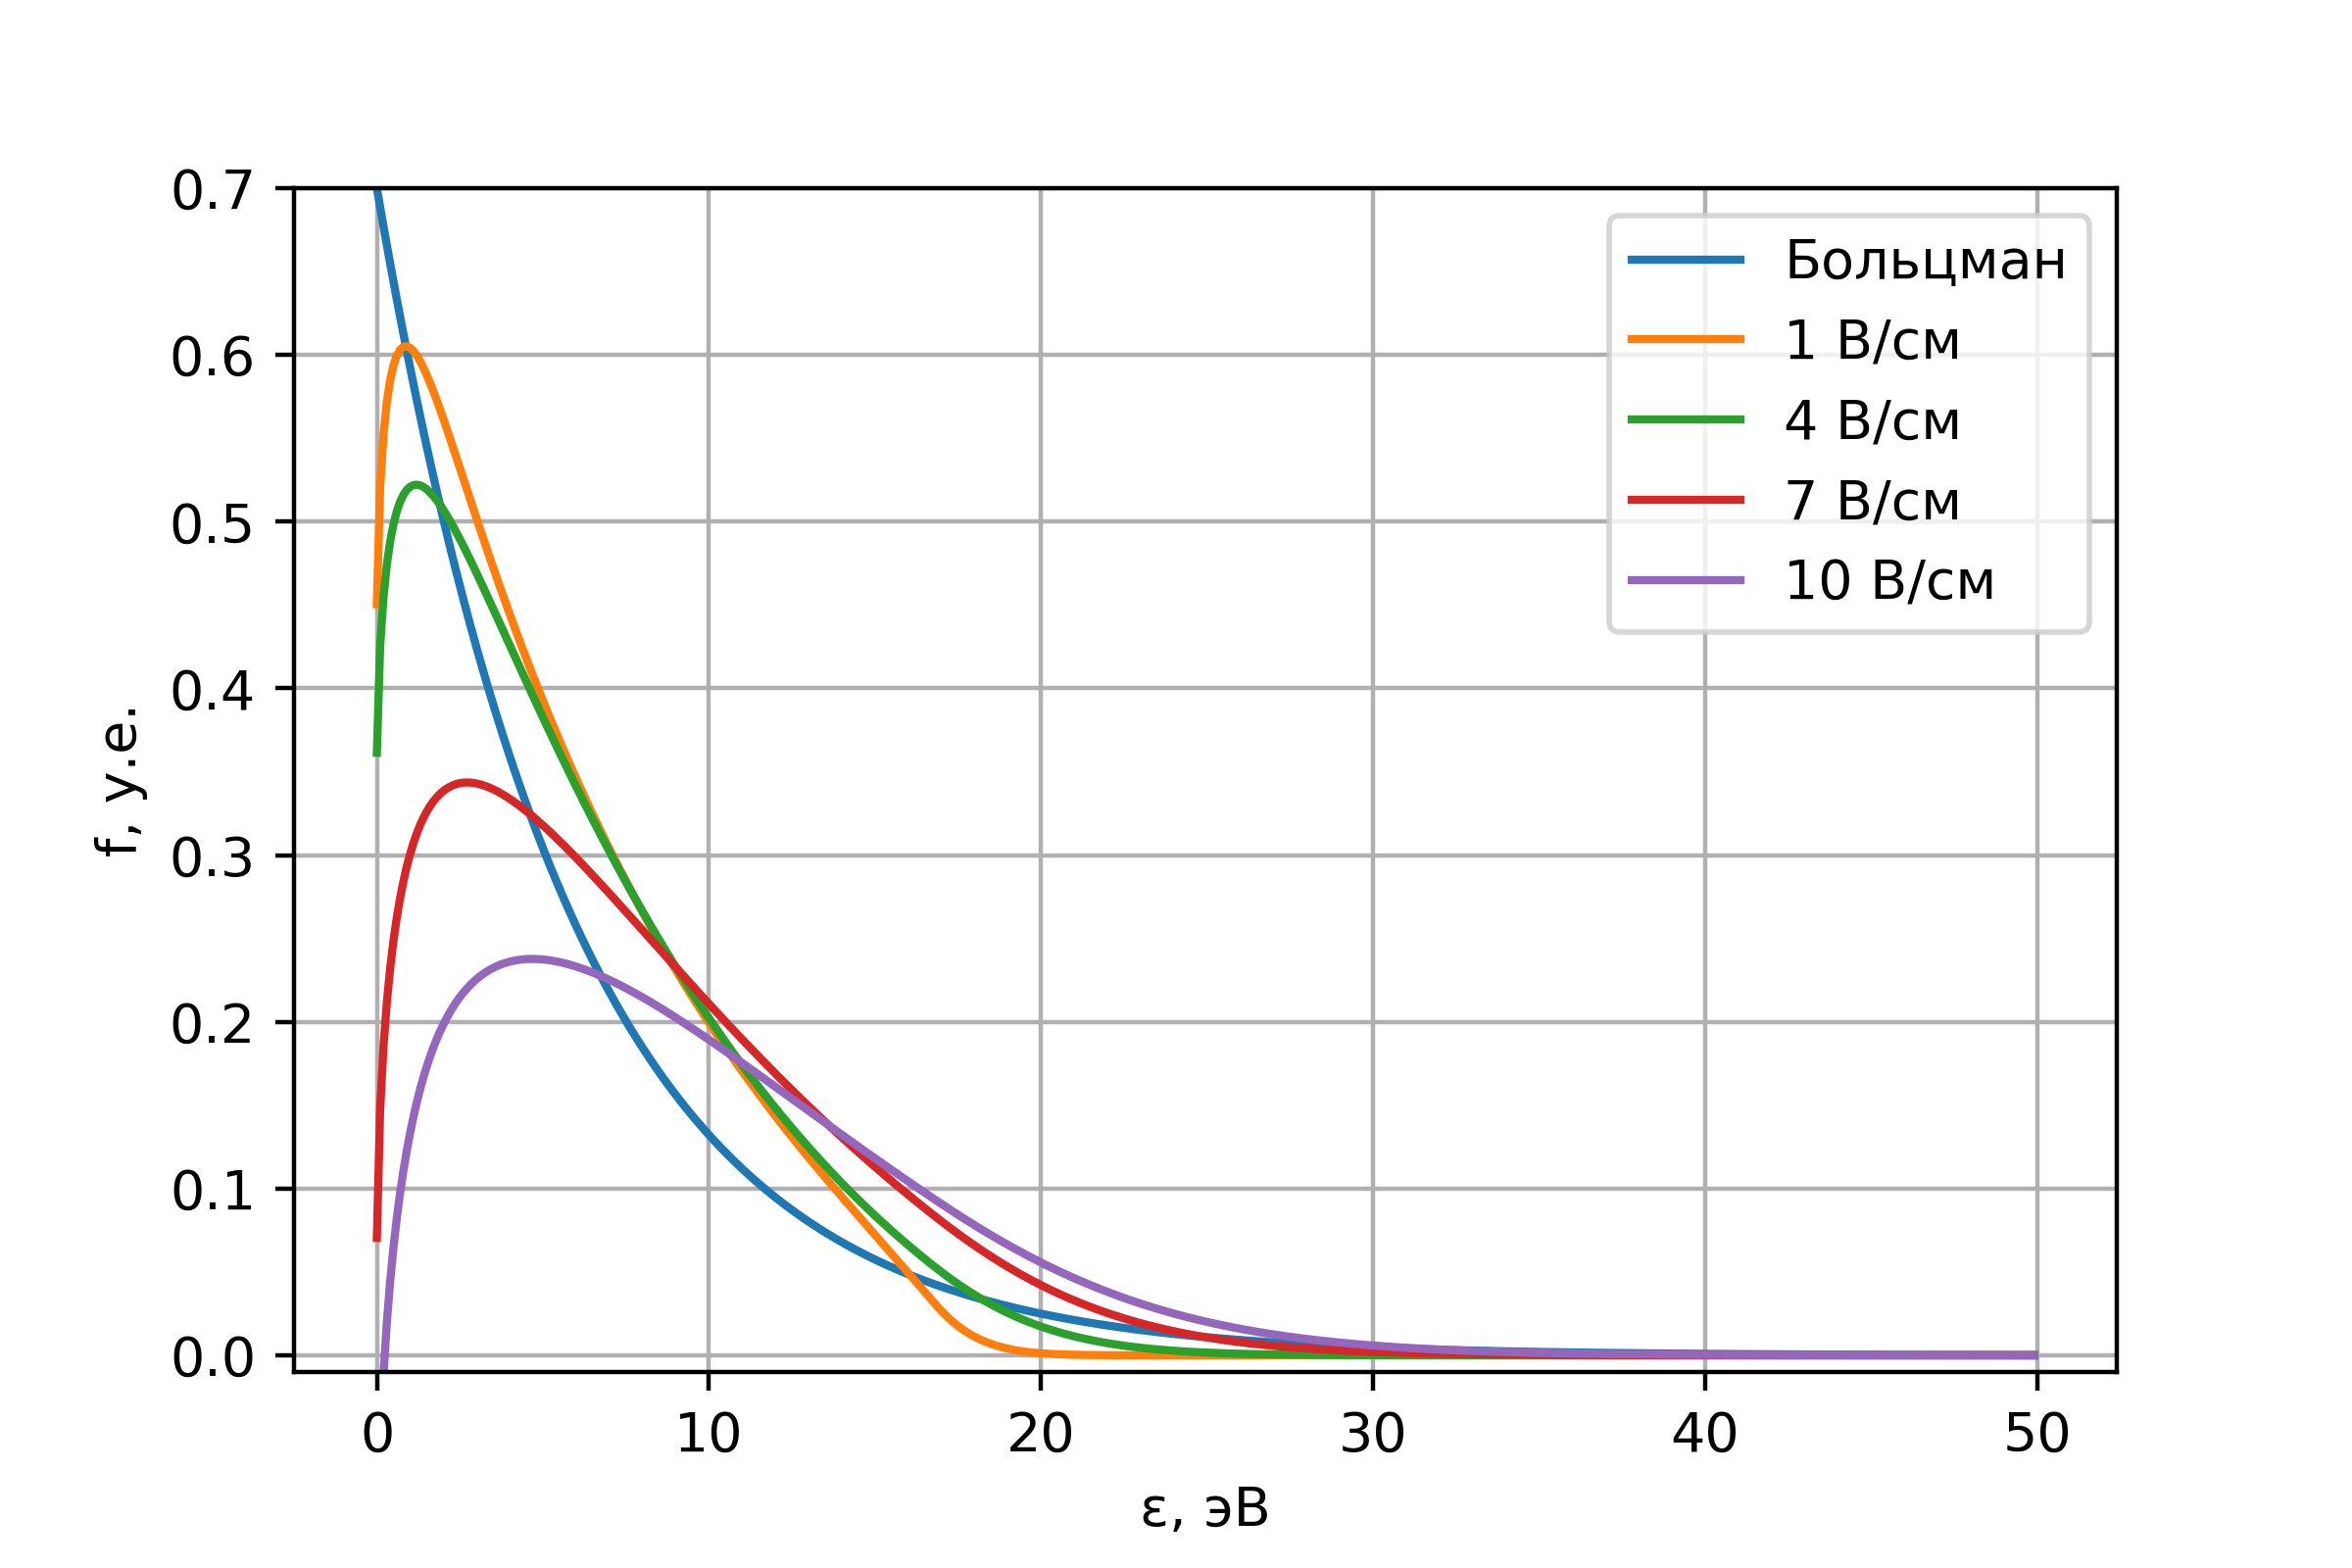
\includegraphics[width=15cm]{figures/fig14}
  \caption{Зависимость расчетной функции распределения электронов от энергии и осевого электрического поля,
  заданного параметрически для некоторых значений.}
  \label{fig:fig14}
\end{figure}

В качестве начальных условий первого вычисления ФРЭ (при \math{E = 1}$~В/см) удобнее всего выбрать распределение
Больцмана, поскольку оно близко к итоговому решению. Удобство заключается в скорости сходимости алгоритма:
чем приближеннее возьмем начальное условие, тем быстрее наступит стационарный уровень.
Затем для расчета ФРЭ для следующего поля лучше всего использовать в качестве начальных условий решение
от предыдущего поля (см.~рис~\ref{fig:fig14}).

Особый интерес в исследовании ФРЭ представляет зависимость в логарифмическом масштабе, поскольку заметить различия
между расчетным распределением и распределением Больцмана на глаз практически невозможно. Распределение Больцмана
в логарифмическом масштабе представляет собой линейную зависимость в отличие от расчетной (см.~рис~\ref{fig:fig15}).
\begin{figure}[t]
    \begin{center}
         \subfloat[\label{sub:fig15a}]{
           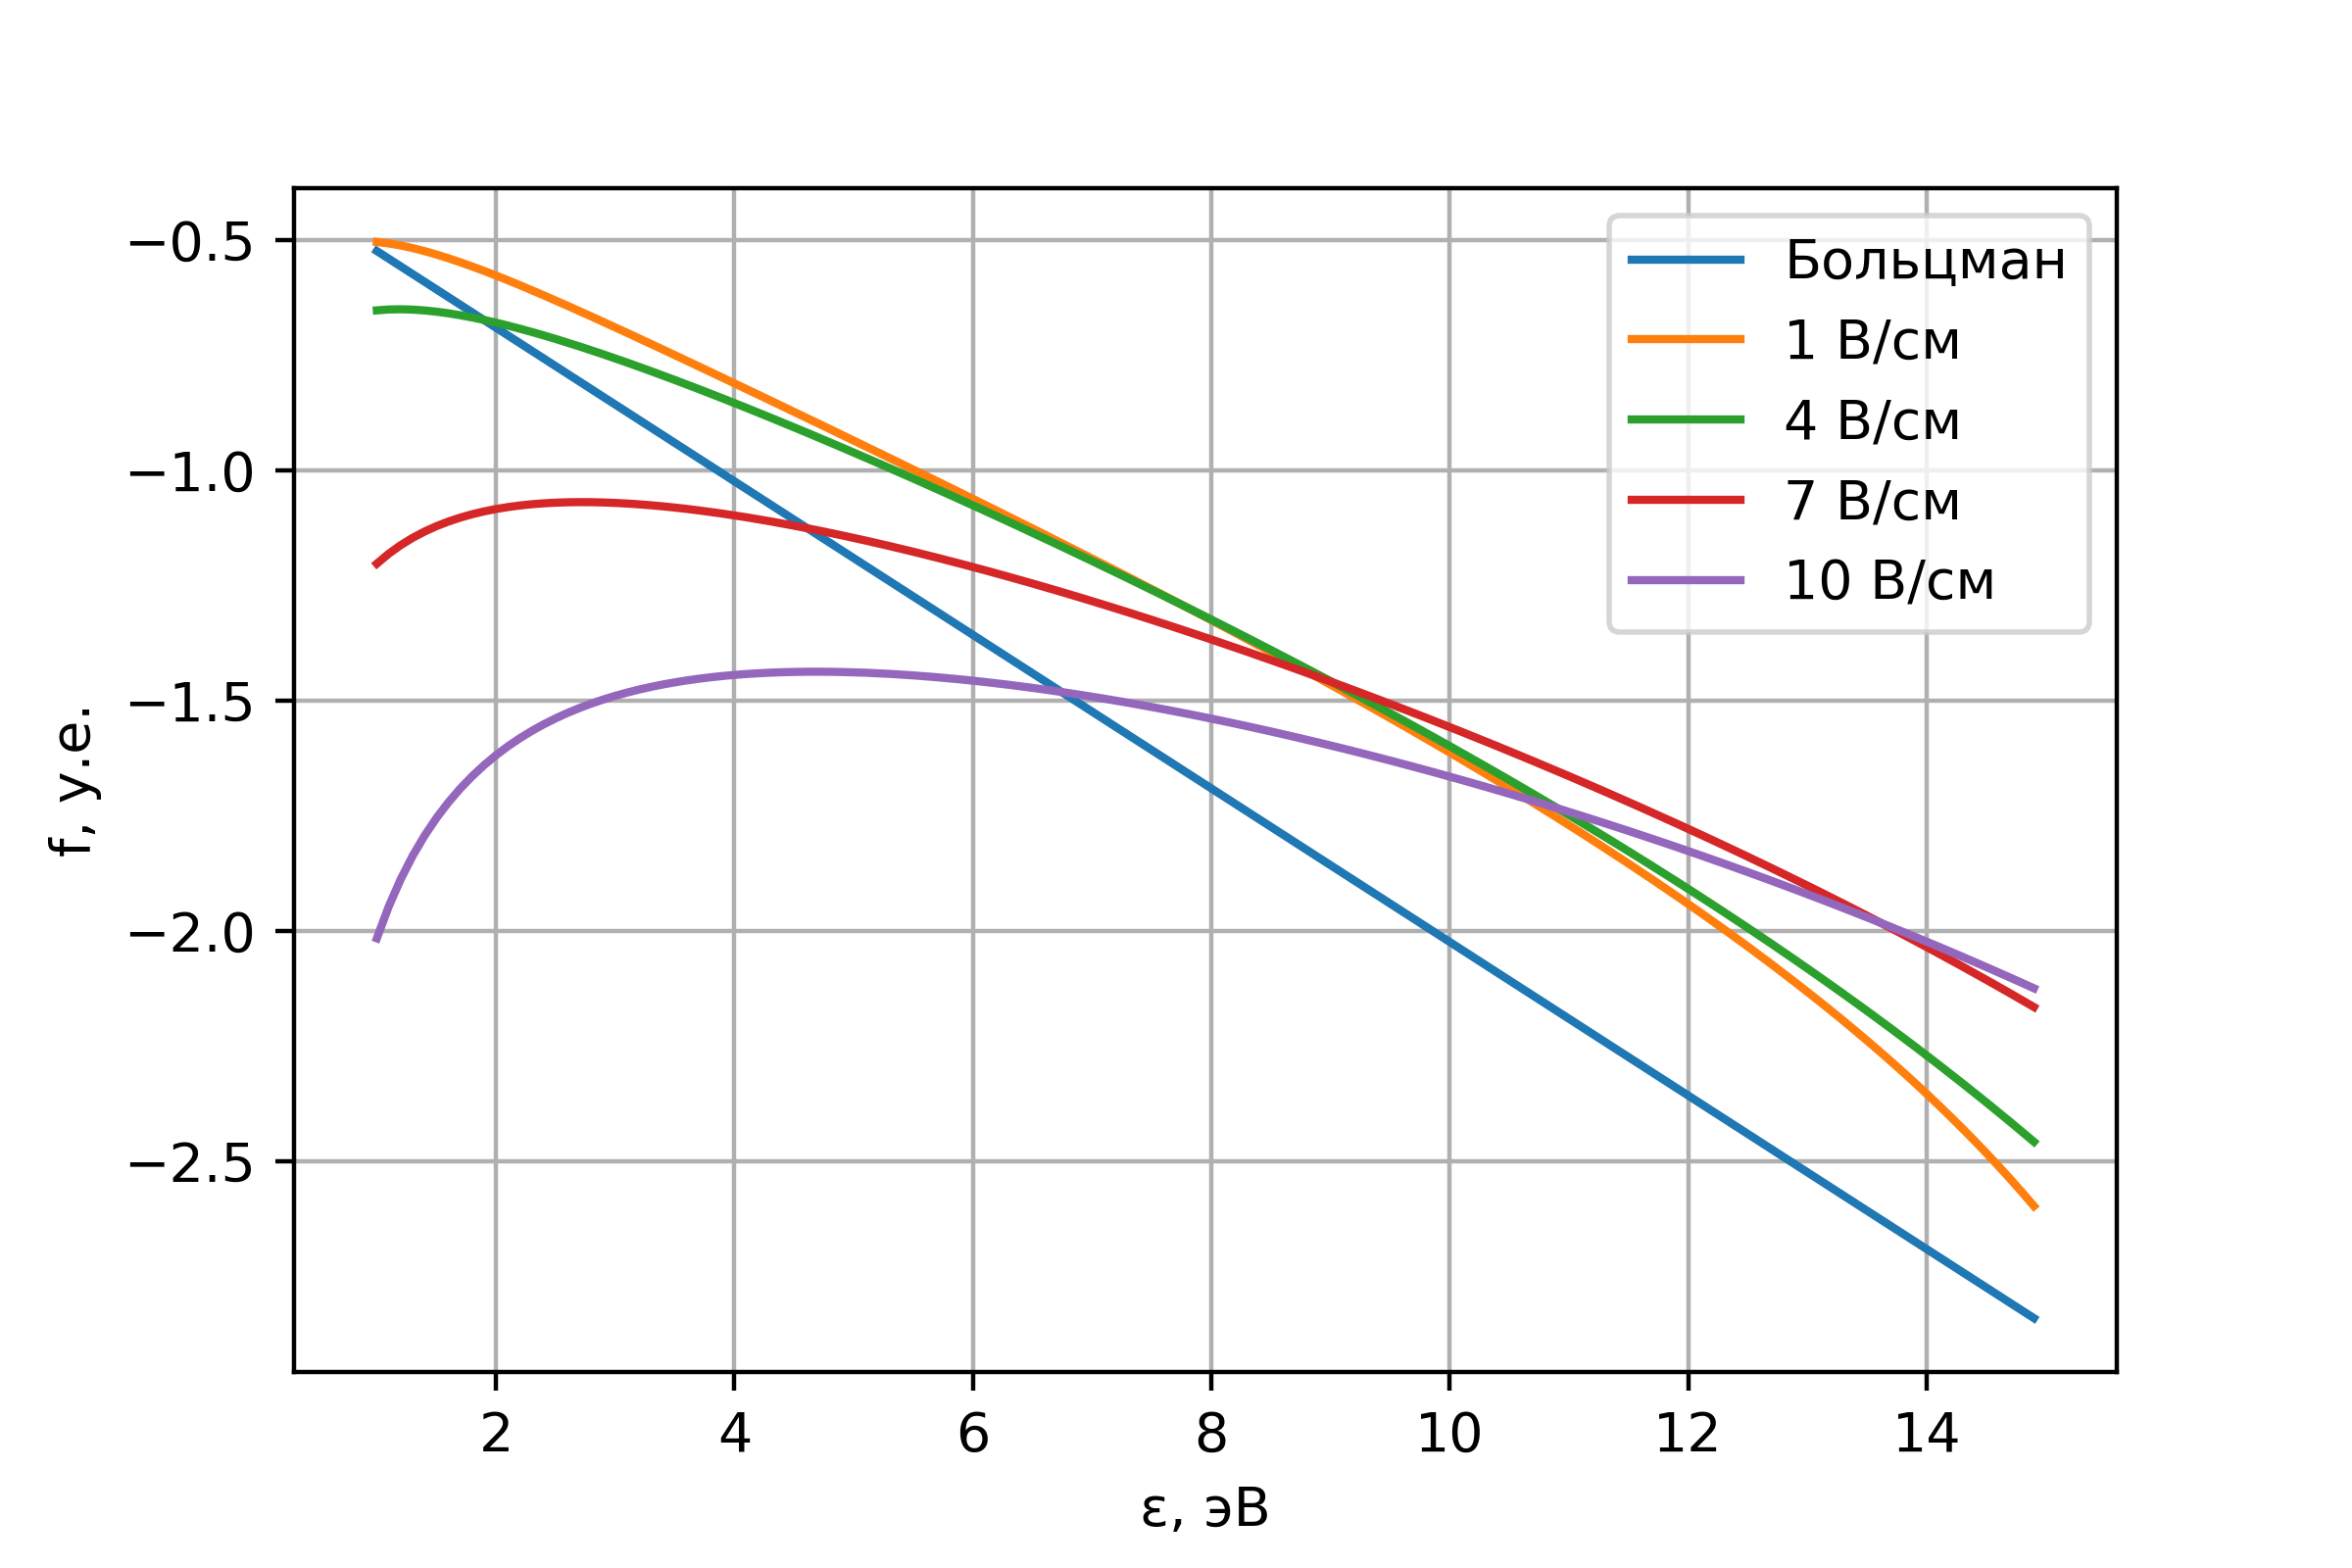
\includegraphics[width=0.49\textwidth]{figures/fig15a}
         }
         \subfloat[\label{sub:fig15b}]{
           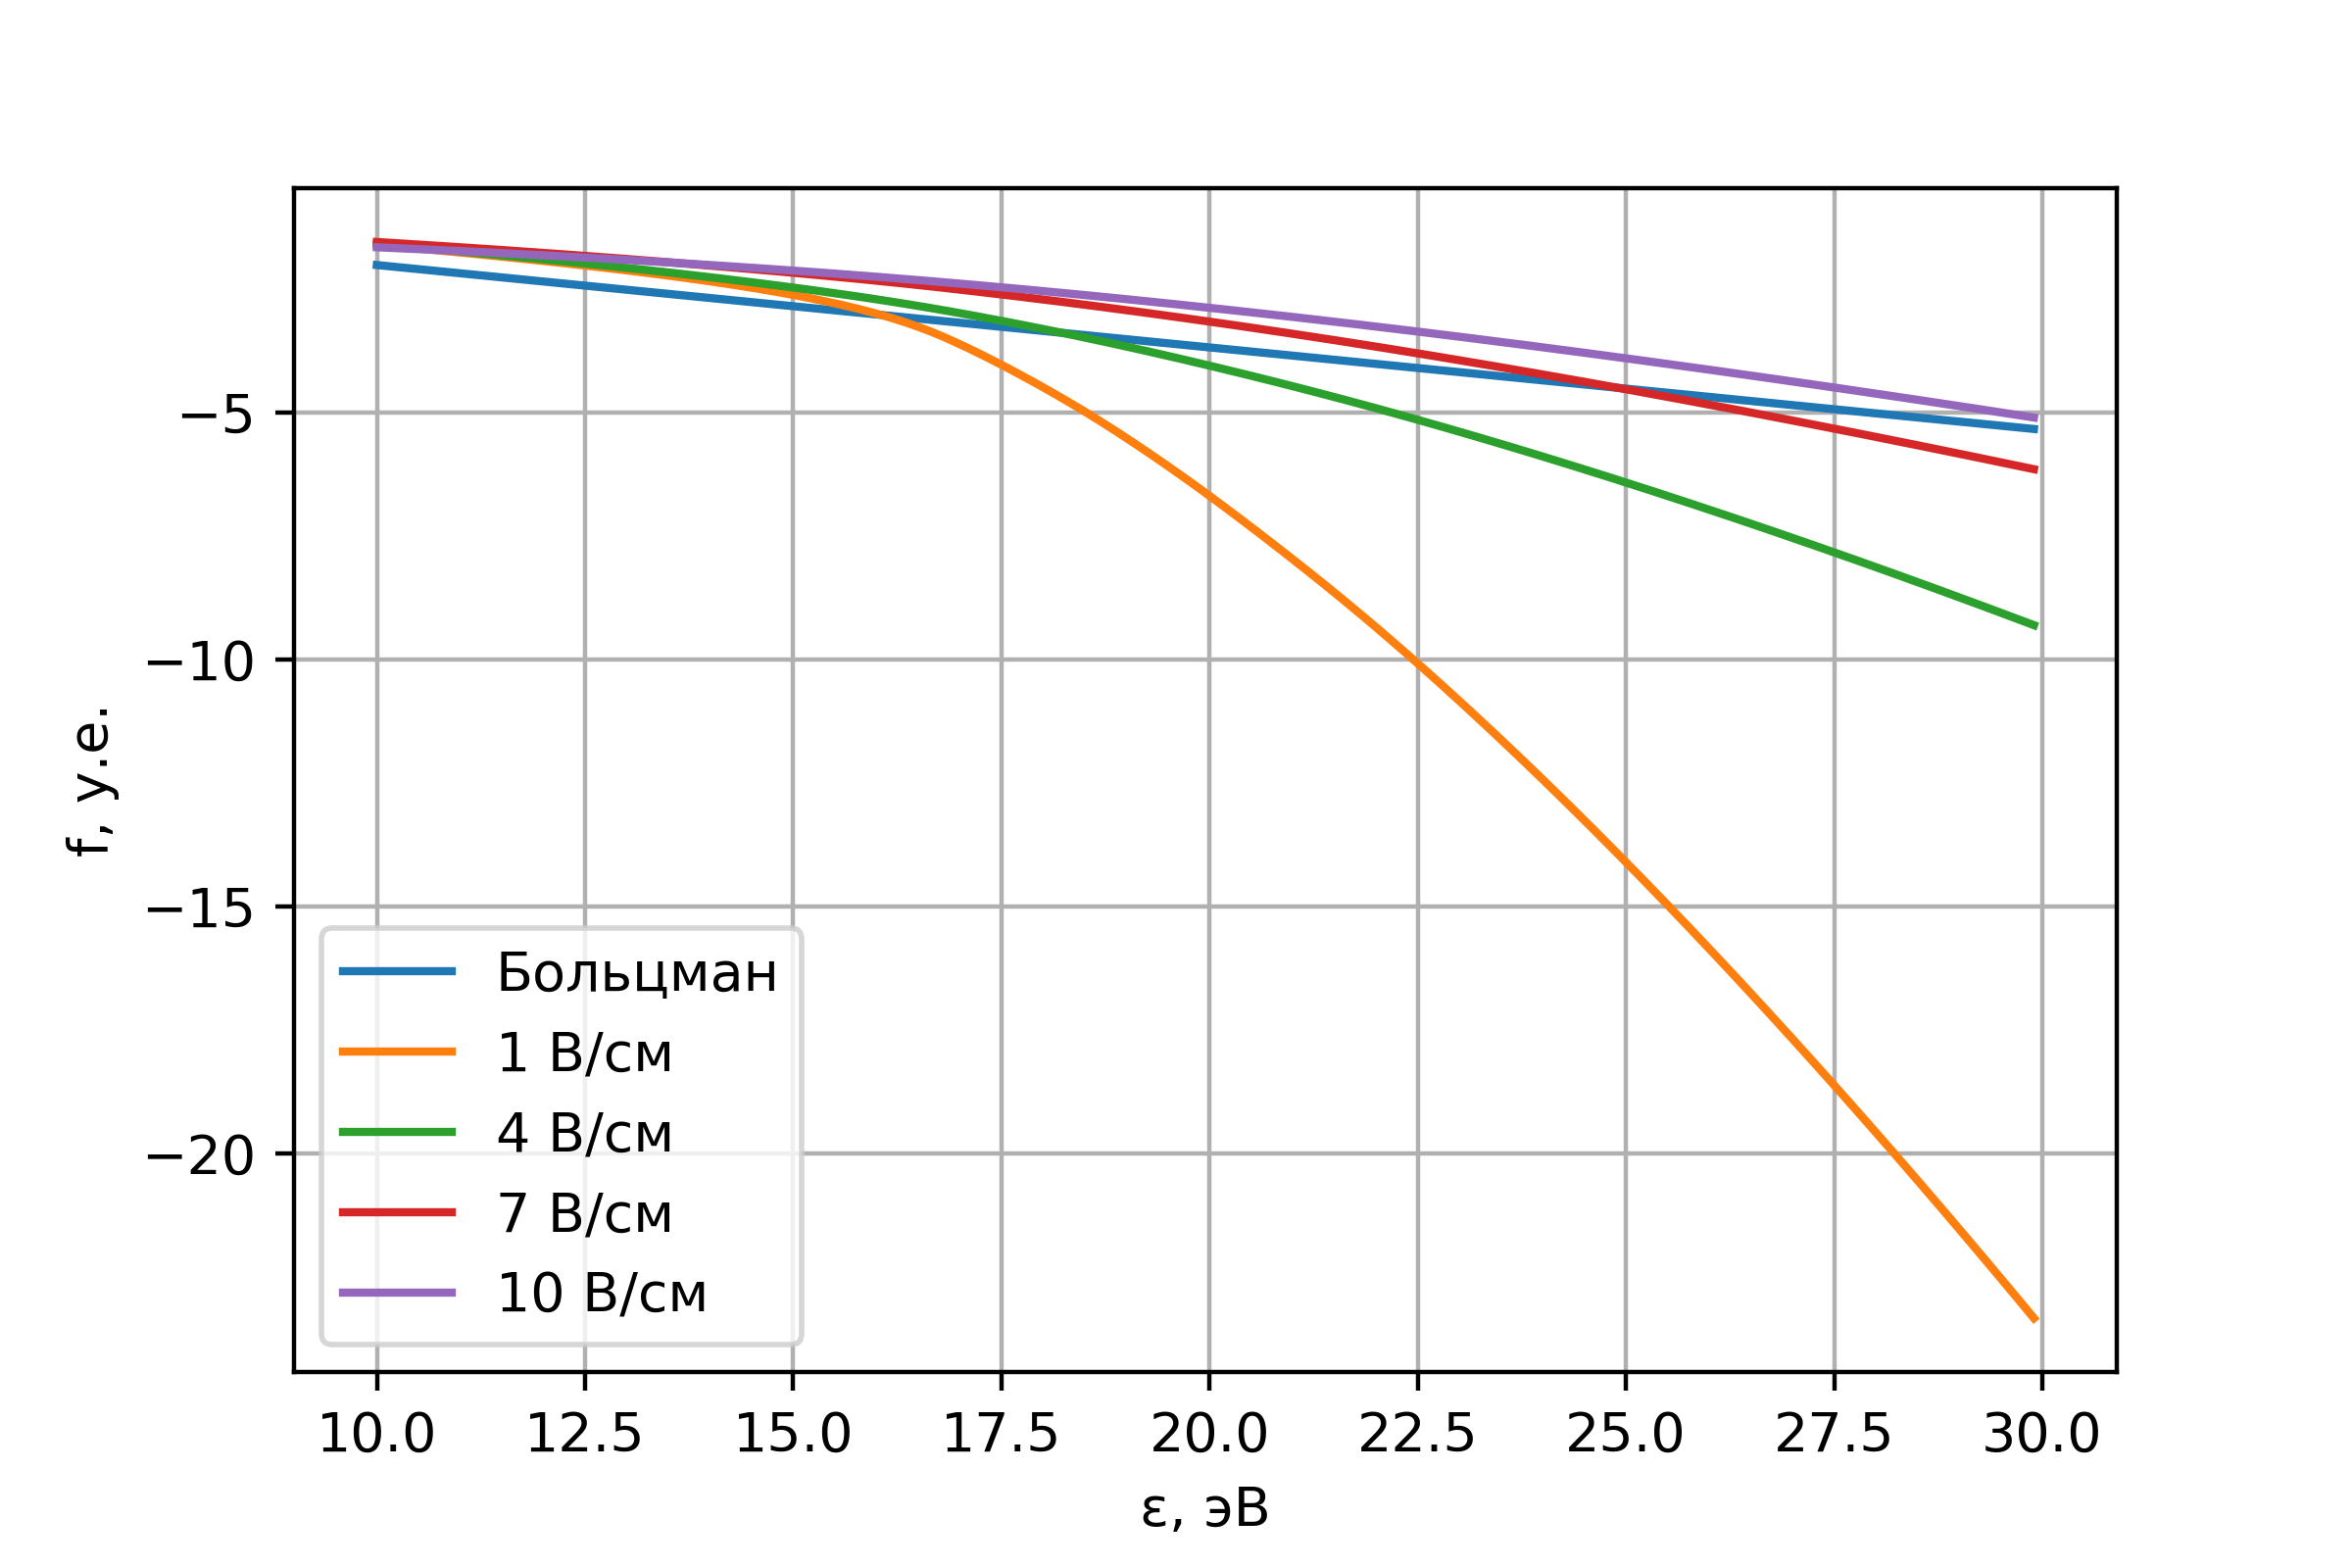
\includegraphics[width=0.49\textwidth]{figures/fig15b}
         }
         \caption{Зависимость расчетной функции распределения электронов от энергии и осевого электрического поля,
                  заданного параметрически для некоторых значений, в логарифмическом масштабе:
                  \pt(a) в диапазоне [1, 15]~эВ, \pt(b) в диапазоне [10, 30]~эВ
         }
         \label{fig:fig15}
    \end{center}
\end{figure}

Из данного графика видно, что расчетная функция распределения электронов принимает двухтемпературный вид.
Это связано с тем, что электроны, имеющие энергию выше пороговой (\math{E_{thr}}$) участвуют в неупругих
столкновениях с атомами.

Поскольку в логарифмическом масштабе функция распределения электронов представляет собой два четко выраженных
линейных участка (двухтемпературный вид), это позволяет рассматривать эти участки независимо друг от друга
со своими электронными температурами:
\begin{equation}
    f_e = e^{-{\epsilon \over T_e}} \Rightarrow ln(f_e) = - {\epsilon \over T_e}
\end{equation}

Зная электронную температуру невозмущенного пылевыми частицами газового разряда, можно определить электронную
температуру с пылевыми частицами из соотношения логарифмов функций распределения энергий:
\begin{equation}
    T_{e,2} = {ln(f_{e,1}) \over ln(f_{e,2})} T_{e,1}
\end{equation}
Для разрешения данного соотношения необходимо понять какие из функций распределения электронов нужно использовать.

Скорость заселения верхних уровней определяется следующим выражением:
\begin{equation}
    X_{exc} (T_e) = \sqrt{2 \over m_e} \int_{E_{th}}^{\infty} \sigma(\epsilon)f_e(\epsilon)\sqrt{\epsilon}d\epsilon
\end{equation}
где \math{\sigma (\epsilon)}$~--~сечение (вероятность перехода) в зависимости от энергии
\math{f_e (\epsilon)}$~--~функция распределения электронов по энергиям

\begin{figure}[t]
  \centering
  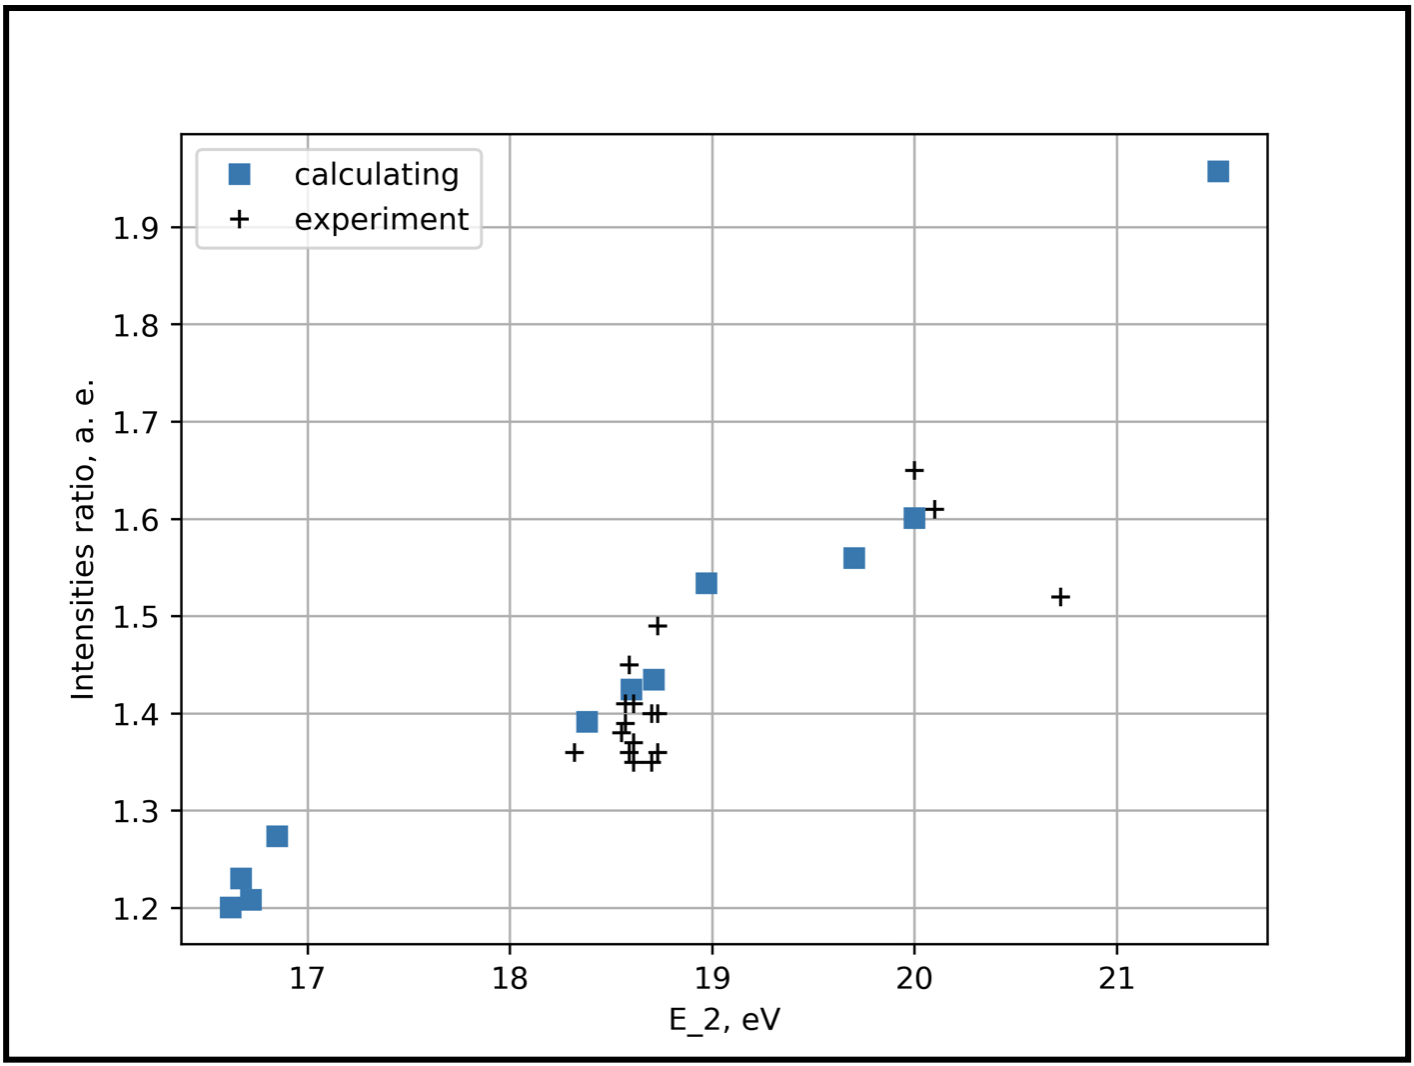
\includegraphics[width=12cm]{figures/fig16}
  \caption{Зависимость ...... .}
  \label{fig:fig16}
\end{figure}

В рамках одного и того же переходного процесса справедливы следующие рассуждения: интенсивность
спектральной линии пропорциональна заселенности верхнего уровня данного перехода, которая в свою очередь
пропорциональна скорости заселения верхнего уровня, т. е.:
\begin{equation}
I(T_e) \sim N^*(T_e) \sim X_{exc}(T_e) \sim  \int_{E_{th}}^{\infty} \sigma(\epsilon)f_e(\epsilon)\sqrt{\epsilon}d\epsilon
\end{equation}

Перейдя к отношению интенсивностей:
\begin{equation}
{{I_2} \over {I_1}}= {{\int_{E_{th}}^{\infty} \sigma(\epsilon)f_{e,2}(\epsilon)\sqrt{\epsilon}d\epsilon} \over
{\int_{E_{th}}^{\infty} \sigma(\epsilon)f_{e,1}(\epsilon)\sqrt{\epsilon}d\epsilon}}
\end{equation}

Из последнего выражения можно сделать вывод, что отношение интенсивностей задается функцией распределения электронов,
а также энергией верхнего уровня. Узнав значение функции распределения электронов для различных значений энергий в
зависимости от кинетических параметров, а также выбрав  фиксированную линию, можно на основе измеренных значений
отношений интенсивностей узнать относительное изменение кинетических параметров системы, таких как электронная
температура и осевое электрическое поле.

Следует отметить, что энергия верхнего уровня влияет на значение отношения интенсивностей, что мы и наблюдаем в эксперименте.

Для невозмущенного состояния исследуемого газового разряда осевое поле было получено из работ […]
и составляет 2.2~В/см, что дает возможность определить ФРЭ \math{f_{e,1}}$. Были перебраны все расчетные функции
распределения электронов и выбрана та, которая наиболее близко приближает экспериментальные отношения
интенсивностей (см.~рис~\ref{fig:fig16}).

Были получены следующие значения:

